\mode<article>

Una vez obtenida la distribución de temperaturas,
podemos medir, por ejemplo, los flujos de calor 
que de ella se derivan.  Como sabemos, los flujos de
calor son proporcionales a la derivada primera de 
la temperatura. En los nodos interiores, es posible
aproximar esta derivada por un cociente incremental
centrado como se esquematiza en la figura \ref{FiguraFlujosCalorAdentro}.
 Sin embargo, en los bordes es necesario tomar
 algunos cuidados. Por ejemplo, es posible optar
 por tomar cocientes incrementales hacia la derecha
 para los nodos en el bordeizquierdo, etc. 

Pueden utilizarse varios métodos para visualizar 
los campos vectoriales como el flujo, pero en 
general es necesario ejecutar una instrucción 
cuyos argumentos serán las posiciones a las que
corresponden cada vector, y las componentes 
$x$ e $y$ para cada punto del recinto calculado.
El resultado se muestra en la Figura \ref{FiguraResultadosFlujos}

\begin{figure}
  \includeslide[width=\textwidth]{FrameFlujosCalorAdentro}
  \caption{Derivadas Primeras para los nodos interiores 
  y del borde. \label{FiguraFlujosCalorAdentro}}
\end{figure}

\begin{figure}
  \includeslide[width=\textwidth]{FrameResultadosFlujos}
  \caption{Resultado final incluyendo el flujo de calor para 
  las condiciones de borde de temperatura \label{FiguraResultadosFlujos}
  }
\end{figure}

\mode*
\begin{frame}<presentation>[label=FrameFlujosCalorAdentro]
  \frametitle{Cálculo de los Flujos de Calor}
    \tikzset{dT/.style={->,>=latex,line width=2pt}}
    \tikzset{dy/.style={alt=<beamer>{draw=Blue},alt=<handout>{draw=DarkRed}}}
    \tikzset{dx/.style={draw=Blue}}
  \begin{columns}
    \column{0.7\textwidth}
    \centering
    \begin{tikzpicture}
    \draw [line width=1pt] (-2,-2) grid (2,2);
    \foreach \x in {-2,...,2}
    	\foreach \y in {-2,...,2}
	{
	  \draw [fill=black] (\x,\y) circle (2pt);
	  }
      \draw [draw=none,fill=black,minimum height=1pt] (0,0) circle (2pt); 
      \draw [ dashed, draw=DarkGreen, line width=2pt ] (-1.5,-1.5) rectangle (1.5,1.5);
      \draw<2> [dT, draw=Blue ] (-1,0) -- (1,0) ;
      \draw<3> [dT,dy] (0,-1) -- (0,1) ;
      \node [draw=none,fill=black, circle,minimum height=1pt] at (0,0){};
  \end{tikzpicture}

    \vspace{1cm}
    \onslide<2>
    \tikz[baseline]\draw[dT,dx] (-0.5,0) -- (0,0) ;
    $Q_x \propto \frac{\partial T}{\partial x} = \frac{T_{k+1} - T_{k-1}}{2 \Delta x}$
    \hspace{1cm}

    \onslide<3>
    \tikz[baseline]\draw[dT,dy] (0,0) -- (0,0.5);
    $ Q_y \propto \frac{\partial T}{\partial y} =  \frac{T_{k+N_x} - T_{k-N_x}}{2 \Delta y}$
    \hspace{1cm}

    \column{0.4\textwidth}

    \onslide<1->
    \begin{tikzpicture}
      \draw ( -1,-2) grid (0.5,2);
      \foreach \x in {-1,0}
          \foreach \y in {-2,...,2}
	  { \draw [fill=black] (\x,\y) circle (2pt) ; }
	  \draw<2>[dT,dx] (-1,0) -- ( 0,0) ;
	  \draw<3>[dT,dy] (0,-2) -- ( 0,-1) ;
    \end{tikzpicture}


    \vspace{1cm}
    \onslide<2>
    \tikz[baseline]\draw[dT,dx] (-0.5,0) -- (0,0) ;
    $Q_x \propto \frac{\partial T}{\partial x} = \frac{T_{k+1} - T_{k}}{ \Delta x}$

    \onslide<3>
    \tikz[baseline]\draw[dT,dy] (0,0) -- (0,0.5);
    $ Q_y \propto \frac{\partial T}{\partial y} =  \frac{T_{k+N_x} - T_{k}}{ \Delta y}$
    \hspace{1cm}

  \end{columns}

\end{frame}

\begin{frame}<presentation>[label=FrameResultadosFlujos]

  \frametitle{Resultado Final para Temperaturas Fijas}
  \begin{columns}
    \column{0.4\textwidth}
    
    \includegraphics[width=1.1\textwidth, page=2]{./DATA/Temperaturas-Flujos-1.pdf}

    \column{0.6\textwidth}
      \texttt{MATLAB}
    \begin{codeblock}
      \verbatiminput{./codexamples/streamslice.m}
    \end{codeblock}
      
      \vspace{1cm}
      \texttt{python:}
    \begin{codeblock}
      \verbatiminput{./codexamples/streamlines.py}
    \end{codeblock}
  \end{columns}


\end{frame}
\mode<all>
